\headline{{\textbf{\Large\sffamily Wired for Bonsai}}\\
          {\textbf{YouTube Creators Off\--Camera \& Unfiltered}}}
\label{2025-06-wired}
\noindent
This month on \textit{Wired for Bonsai}, we travel into the analytical yet artistic world of Dutch bonsai artist \textbf{Jelle Ferwerda}. Now living in Germany, Jelle is the mind behind the YouTube channel \textit{Growing Bonsai by Jelle}, where he shares bonsai knowledge shaped by both scientific rigour and hands\--on experience. His quiet voice, calm demeanour, and methodical explanations have guided thousands into the intricacies of bonsai---from wiring and styling to patient long\--term development.

But who is Jelle behind the camera?
What motivates him to keep sharing?
And how does someone trained in ecosystem analysis and plant physiology end up with 300 trees in their garden and a growing international following?

\medskip
\topic{From Childhood Book to Bonsai Obsession}
\noindent
For Jelle, bonsai began as a childhood curiosity. \textit{``I got a little book about bonsai for my birthday,''} he recalls. \textit{``I collected some plants, put them in pots, and then\dots{} over the summer holidays, all of them died.''} It was an early lesson in the unforgiving nature of bonsai---and one that left a mark. He dropped the hobby, moving on with life, but the seed had been planted.

Years later, married and with a house of his own, Jelle returned to the idea. \textit{``It was something I could do near the house, something in line with gardening, which I already enjoyed.''} What began as a gentle pastime quickly took root. \textit{``By now, it influences so much of what I do that you could say it's a lifestyle.''}

And that lifestyle includes more than just a few pots on a bench. Jelle's garden now hosts a sprawling collection of trees---Japanese maples, yews, larches, olives, junipers, and some lesser\--seen species like small\--leaved lilac and true zelkova. Each one a little project. Each one a chapter in his ongoing bonsai story.

\topic{Science, Scepticism \& the Pursuit of Mastery}
\noindent
Jelle is not just a bonsai grower---he's a scientist by training.
With degrees in ecosystem analysis from Wageningen University and a PhD jointly supervised from ITC and Wageningen University and research focusing on plant physiology and remote sensing, his academic background deeply shapes how he engages with bonsai.
\textit{``I question a lot of the so\--called `bonsai facts',''} he says.
\textit{``If I don't understand the reason behind something, I test it. I try different things and see how the tree responds.''}

This curiosity led him to formal bonsai education as well.
He completed an eight\--year course at the International Bonsai School in Düsseldorf, working under renowned teachers Werner Bush and Iwao Katagiri.
\textit{``Each year had a theme---50\% theory, 50\% practice. Every second year we had exams. After six years, you qualify as an independent bonsai artist. After eight, you can teach.''}

Jelle sees this structured path not as restrictive, but as liberating.
\textit{``Going through every step of the process helped me build confidence. Now, I feel comfortable trying things that may not follow the book, because I understand the book first.''}

\begin{window}[%
    2,l,%
    \includegraphics[width=1.0\columnwidth]{2025_06/res/jelle_bonsai_garden},%
    \centerline{\emph{Jelle ``overwintering'' in his garden, surrounded by his trees.}}%
]
\end{window}

\medskip
\topic{Jelle's Approach to Bonsai: Thoughtful, Rooted, and Experimental}
\noindent
Ask Jelle if he sees bonsai as science or art, and he pauses. \textit{``It's such a common question,''} he says. \textit{``If bonsai were just craft, why do we exhibit them like artwork? Why do we have books full of photos but no explanations?''}

He admits he's still in awe of truly artistic trees. \textit{``That's where I struggle---I'm better at development than refinement. Once a tree is in the final stages, I lose interest a bit. I enjoy building something from scratch.''}

\textit{Jelle is currently pushing himself to improve that part of his practice. ``This year's goal is refinement without wire. I'm trying to elevate my trees---make them truly show\--worthy.''}

\topic{Growing Bonsai by Jelle --- YouTube with a Long View}
\noindent
When Jelle started his YouTube channel, it wasn't part of a grand plan. \textit{``I'd just won the German New Talent Contest and someone said, `You need to be online.' So I filmed a video in the dead of winter. To my surprise, it got traction.''}

Since then, he's built a channel that avoids bonsai hype in favour of clarity and continuity. \textit{``My most popular video is about thickening trunks---over 850,000 views. People want foundational knowledge. That's what I try to provide.''}

\begin{window}[%
    2,l,%
    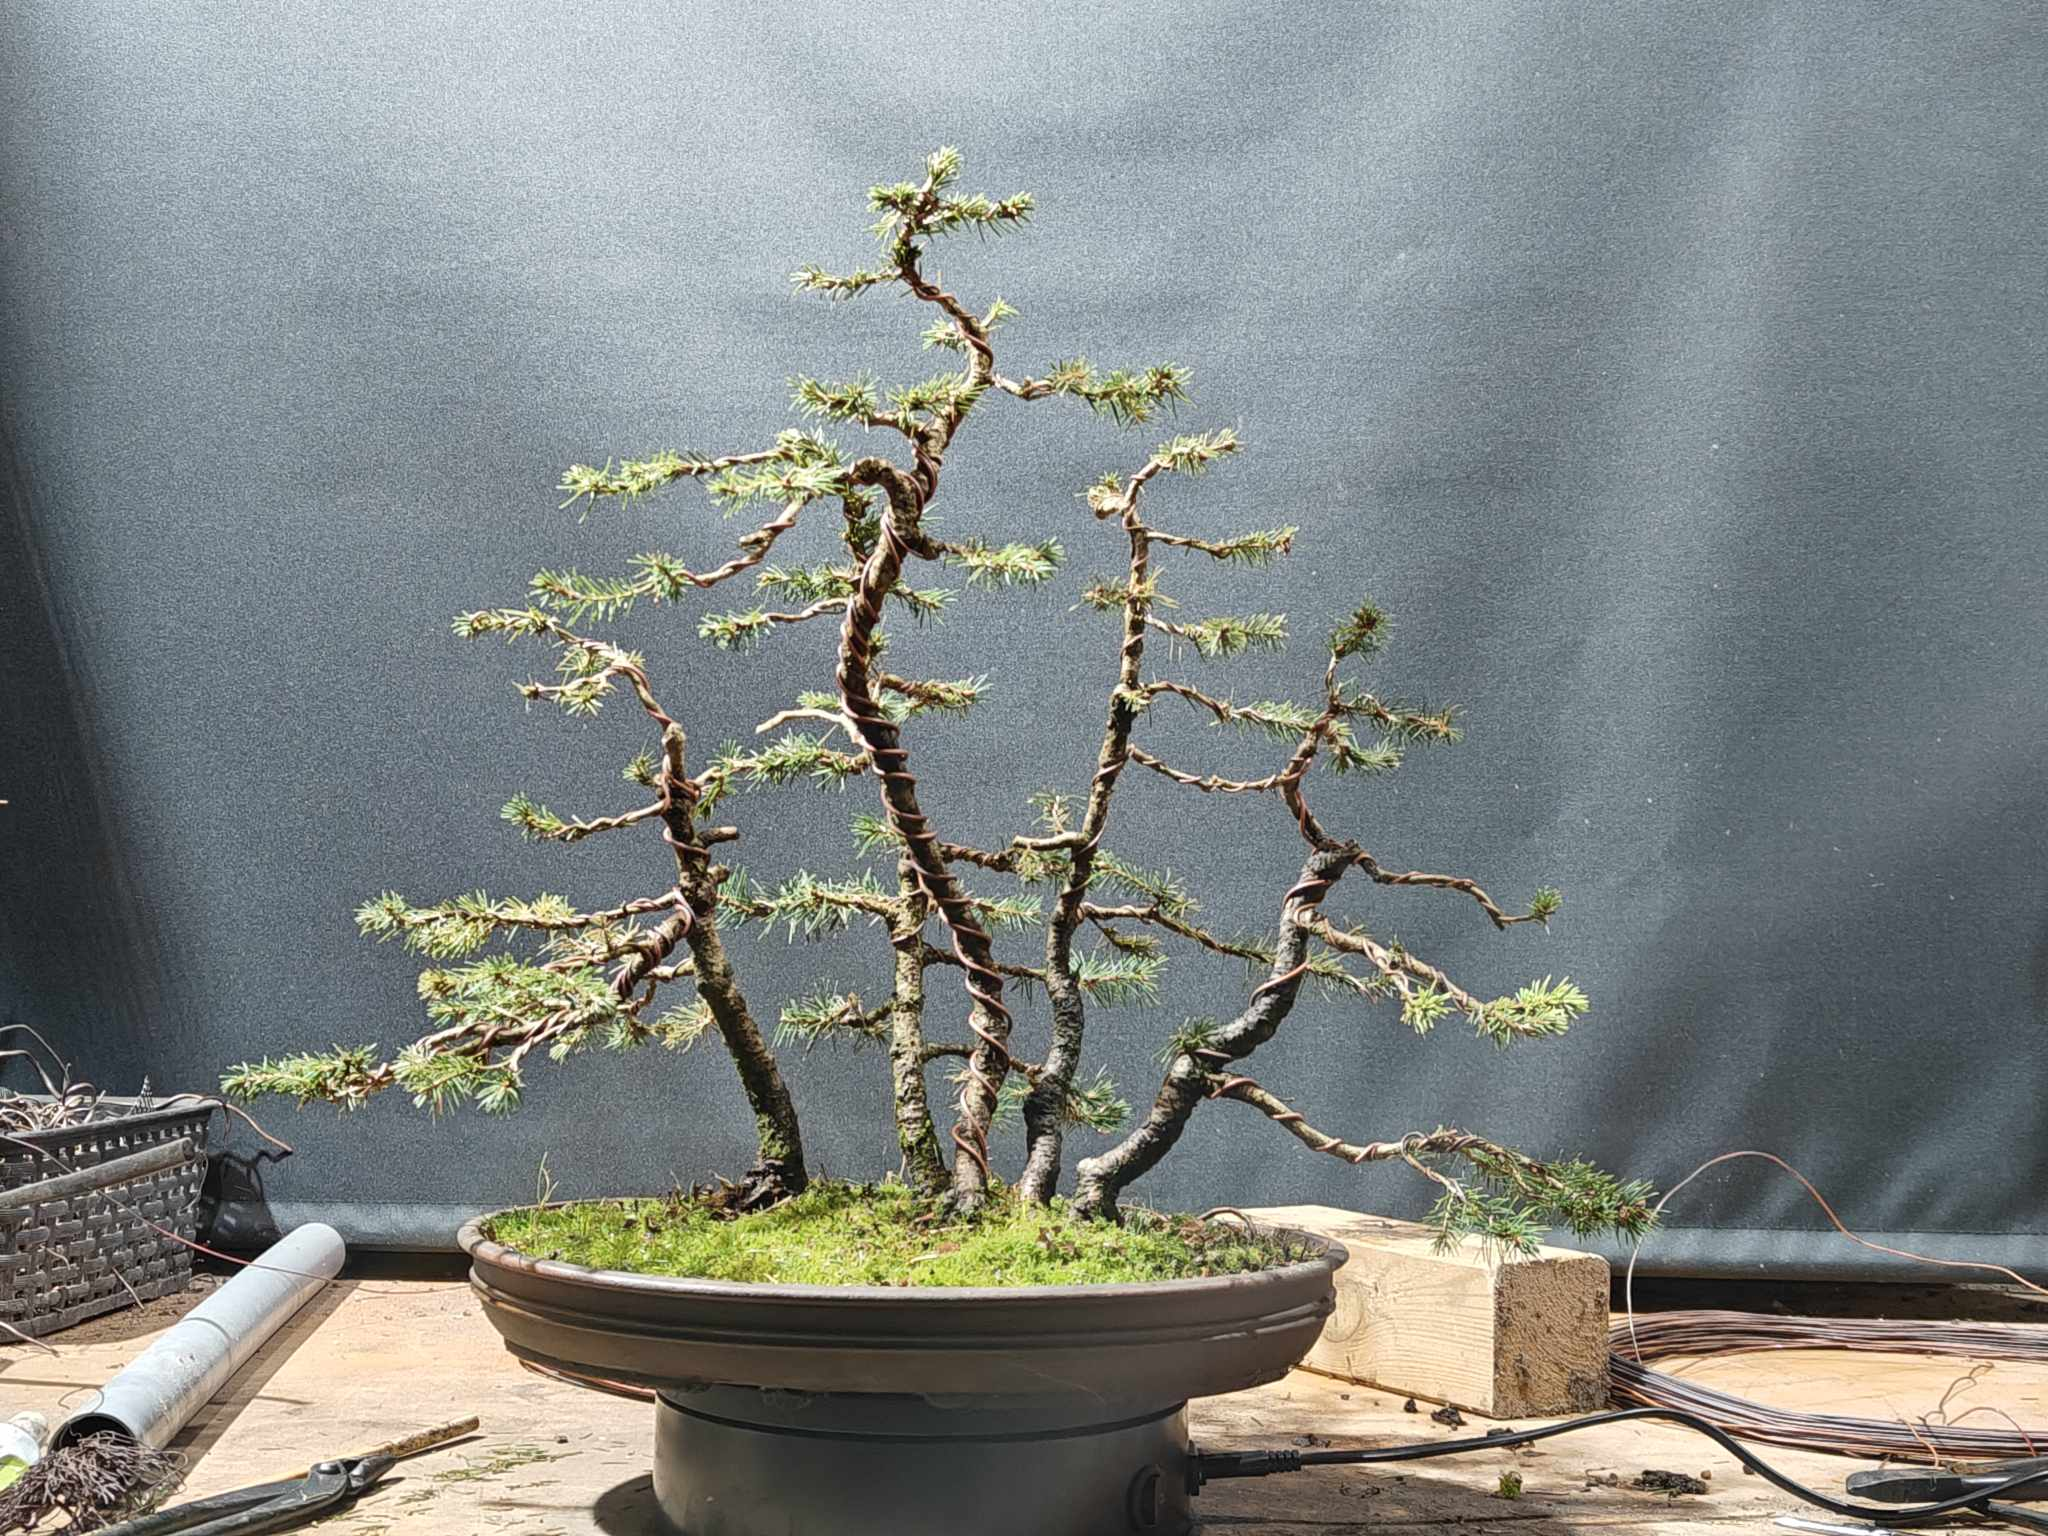
\includegraphics[width=1.0\columnwidth]{2025_06/res/jelle_yew_forest},%
    \centerline{\emph{A developing cedar raft, one of Jelle's major projects.}}%
]
\end{window}
\columnbreak

\begin{window}[%
    2,l,%
    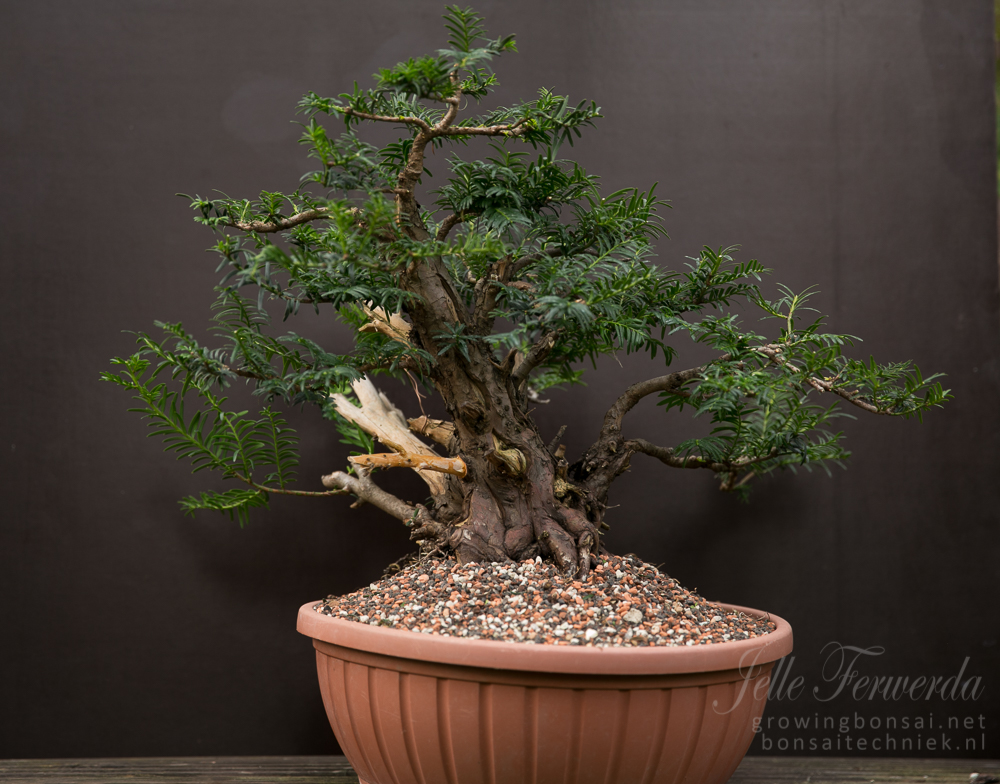
\includegraphics[width=1.0\columnwidth]{2025_06/res/jelle_large_taxus},%
    \centerline{\emph{Jelle's large yew stump trained into bonsai.}}%
]
\end{window}

His videos often span years of footage.
\textit{``Short videos show techniques. But bonsai is about time. I want to show what happens after the technique.''}
That long view has earned him a loyal audience---but also a few trolls.
\textit{``You get insensitive comments. But I try not to let it get to me. Most people are incredibly kind.''}

\medskip
\topic{In the Garden --- Work in Progress}
\noindent
Behind the camera, Jelle's bonsai garden is always evolving.
Right now, he's focused on reducing his number of trees.
\textit{``I want fewer trees, but better ones. The temptation is always to add, but I'm working on editing.''}

One of his most exciting projects is a massive pine raft he acquired at the Bonsai Trophy.
\textit{``It's over a metre wide, with five trunks. I'll be working on it with friends---a whole weekend dedicated just to that tree.''}

Like many bonsai artists, he's had his setbacks too.
\textit{``I lost almost the entire canopy of a prized tree this winter. Turns out the pot didn't drain properly. I repotted, and now it's coming back---but I lost ten years of structure.''}

\topic{Clubs, Mentors \& the Power of Honest Feedback}
\noindent
Jelle is a member of several clubs and informal groups.
\textit{``For me, clubs are about sharing knowledge. Not just learning from experts, but listening to the newest members too. Everyone brings something different.''}

He's had formative experiences with teachers like Mr. Katagiri and artists like Werner Busch, Pavel Slovák, and even the UK's own Tony Tickle.
\textit{``Those early workshops changed how I think about bonsai.''}

But mentorship doesn't have to be formal.
\textit{``You need someone who'll tell you when your tree is rubbish. We all think our own trees are great---but having someone keep you grounded is essential.''}

\begin{window}[%
    2,l,%
    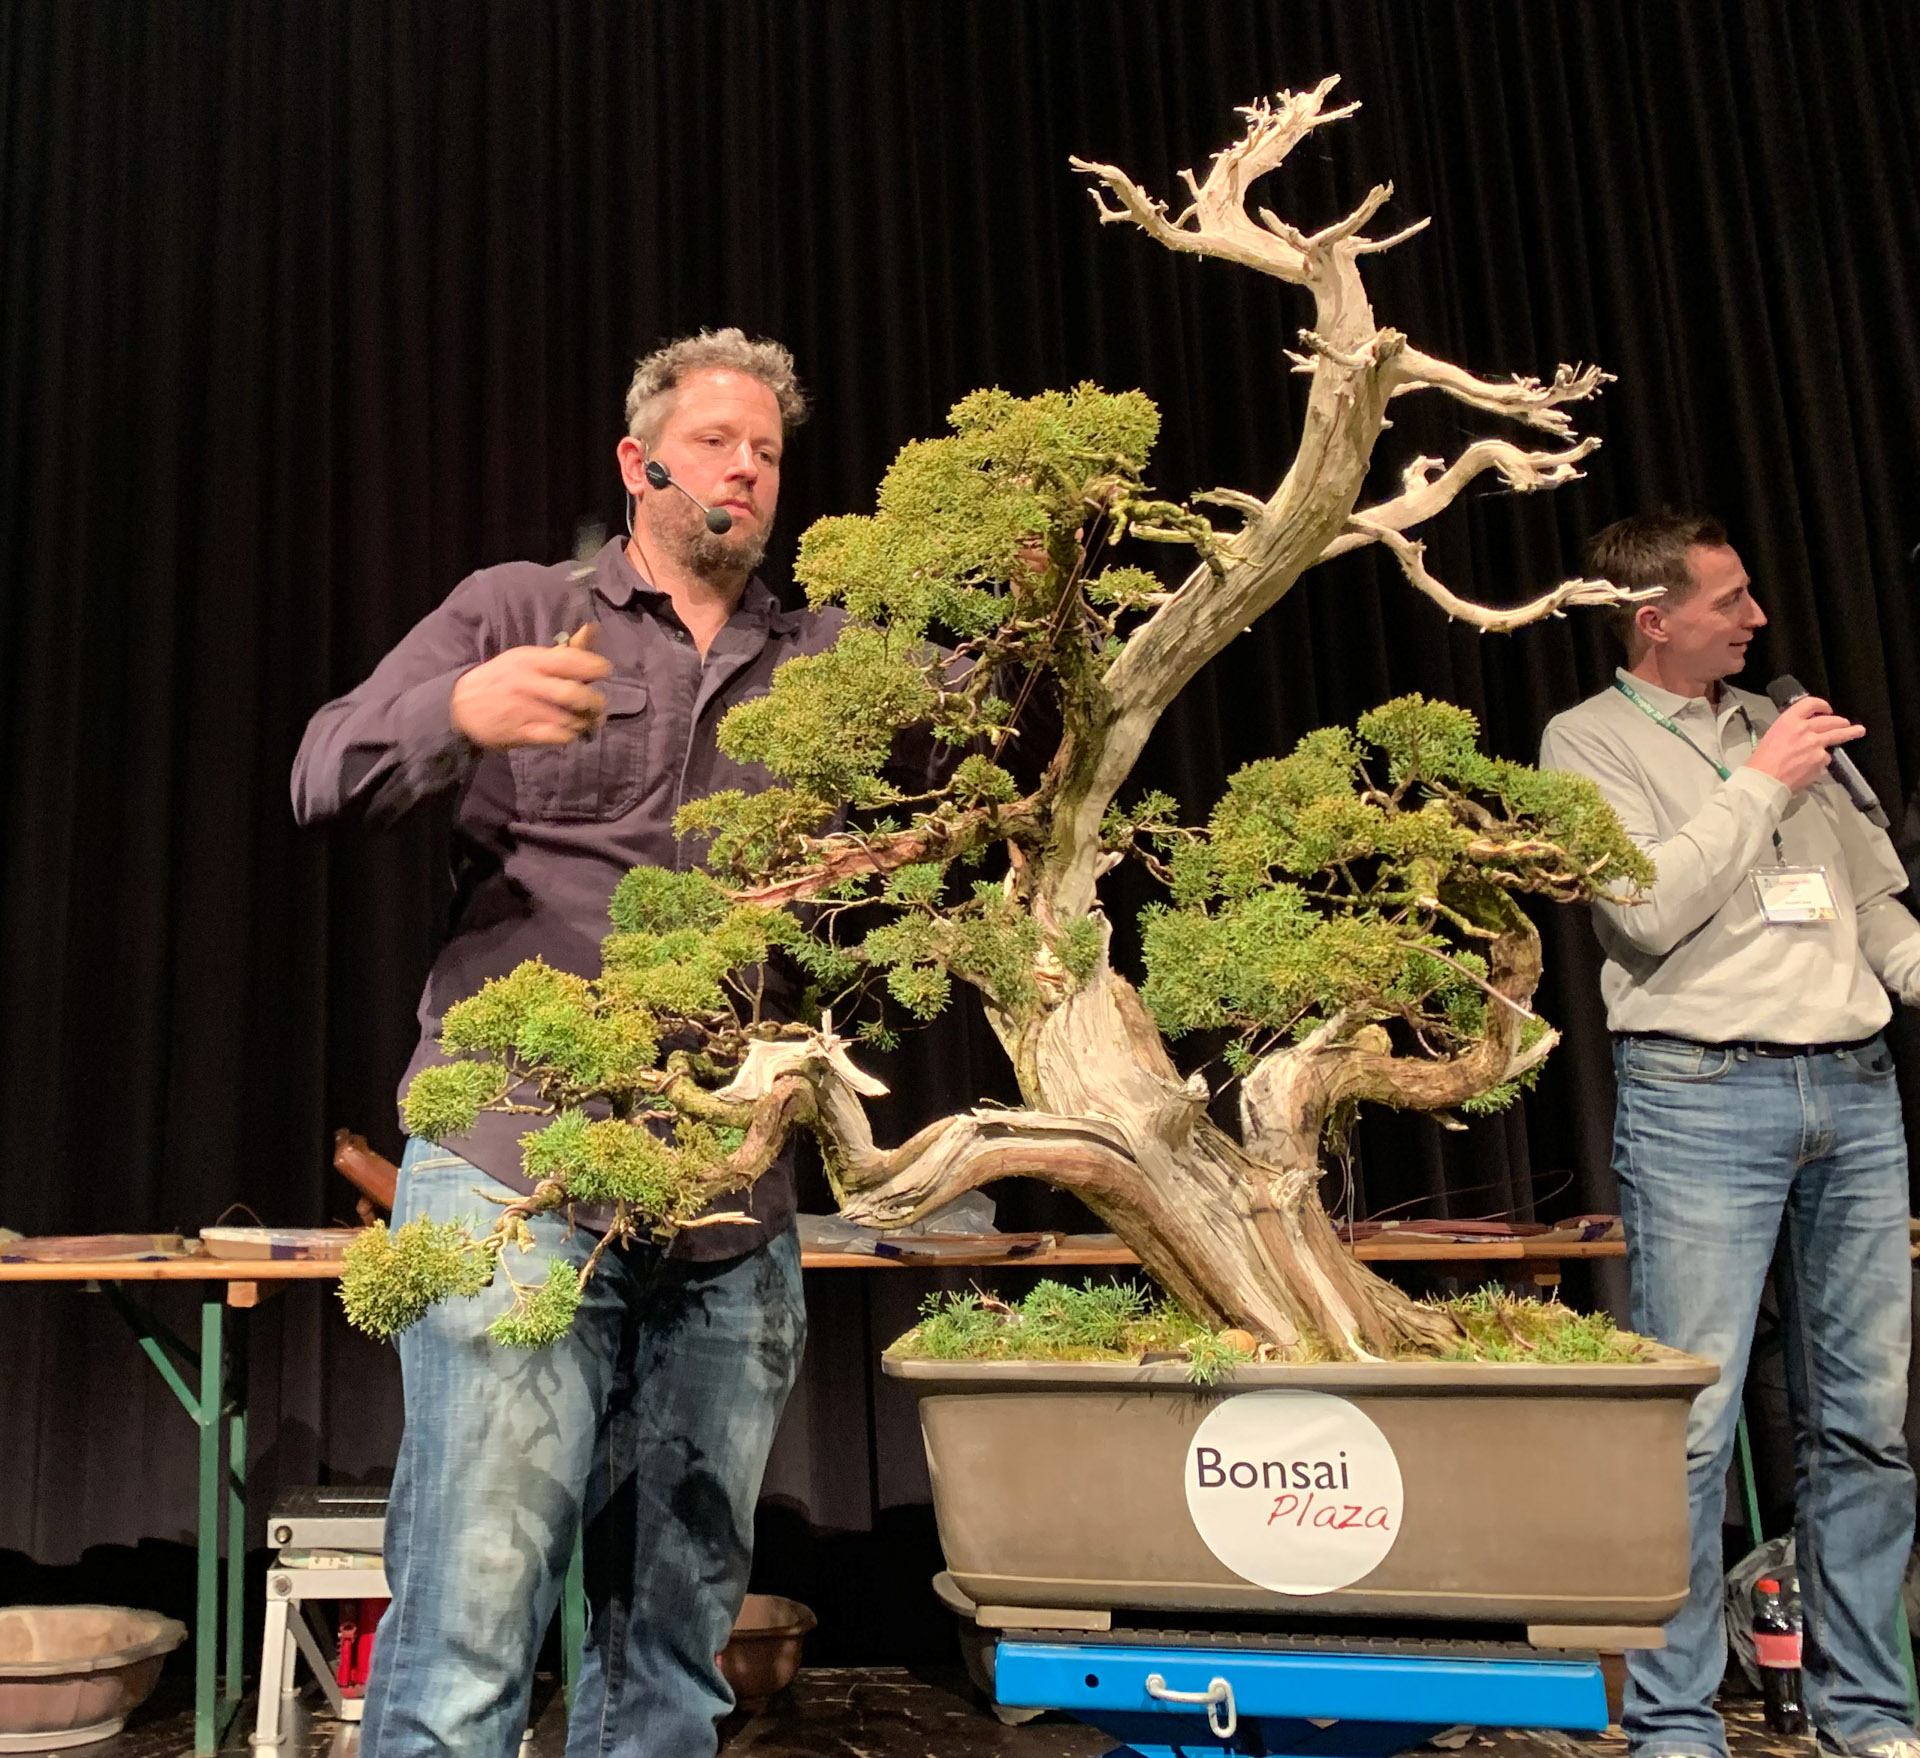
\includegraphics[width=1.0\columnwidth]{2025_06/res/jelle_trophy_25},%
    \centerline{\emph{Jelle assisting Ryan Neil with a large juniper at Trophy '25.}}%
]
\end{window}

\medskip
\topic{Looking Forward --- Quietly Ambitious}
\noindent
Despite his low\--key demeanour, Jelle has clear goals.
\textit{``This year I'm showing trees at three exhibitions, including the German national show. I'd love to get trees into top\--tier European events like the Trophy.''}

He's also toying with the idea of a book.
\textit{``I've written a 50\--page beginner's manual for my club. There's a gap for a practical, modern guide. Who knows, maybe I'll publish it.''}

And his advice for beginners?
\textit{``Start with cheap trees, get experience, and once you know how to keep them alive, buy good trunks. Growing a bonsai takes ten years. Maturing it takes another ten. The sooner you start, the better.''}

So, in the end, how would you capture the essence of bonsai in a single word?
\textit{``Passion!''}

% \vspace{-3em}
\begin{center}
    $\cdots$
\end{center}
% \vspace{-3em}

\noindent
Jelle Ferwerda isn't just a YouTuber---he's a biologist, an educator, and a student of trees.
His work reminds us that bonsai isn't about quick results.
It's about patience, learning, and above all, staying rooted in the joy of growing.

Check out his channel at \href{https://www.youtube.com/@GrowingBonsaiByJelle}{\textit{Growing Bonsai by Jelle}} and see for yourself how bonsai, done thoughtfully, can become a lifelong adventure.
\closearticle

\vfill
\begin{center}
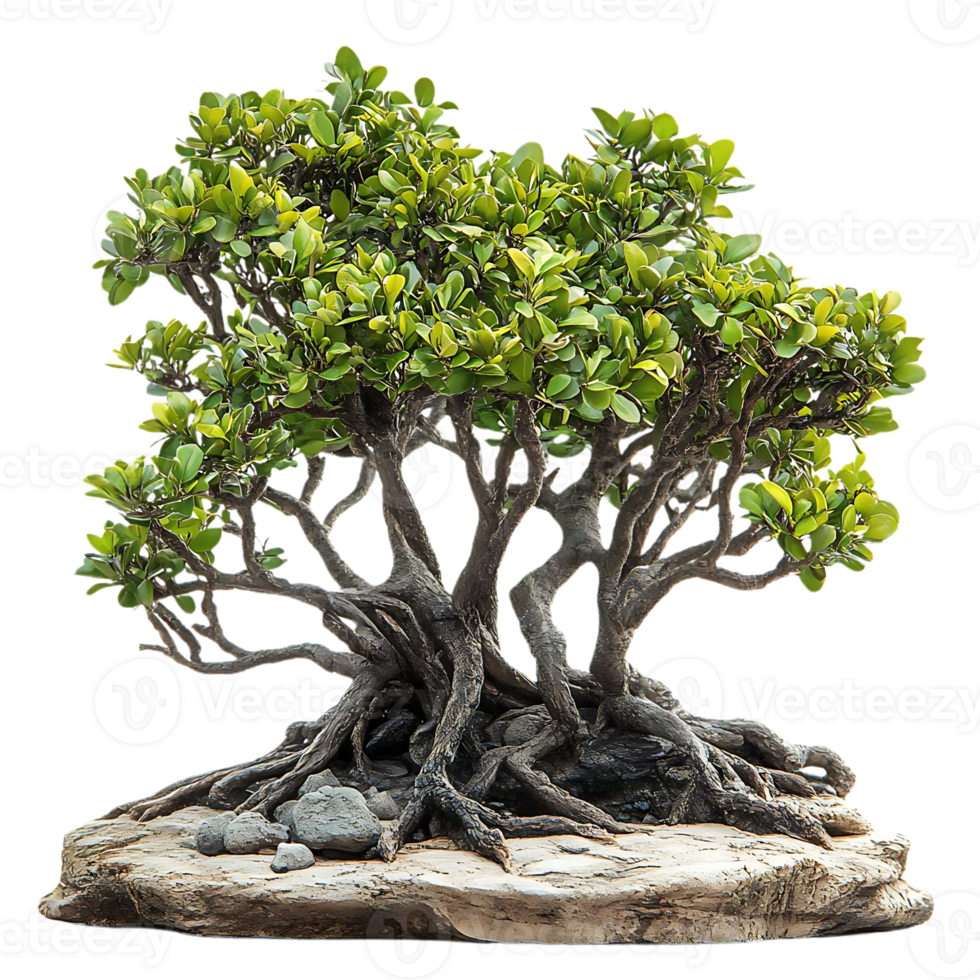
\includegraphics[width=0.3\columnwidth]{res/filler_b}
\end{center}
\pagebreak
